\section{Hypothesis Graph}%
\label{sec:hgraph}
The \acf{hgraph} consists of a set of nodes and edges. Where the node correspond to an object at a configuration, and the edges correspond to actions. As a whole the \ac{hgraph} represents a search (or planned search) in the joint configuration space. The \ac{halgorithm} creates and updates nodes and edges in the \ac{hgraph} and is discussed in \cref{subsec:halgorithm}. A search in the joint configuration space is avoided because an edge only operates in a single mode of dynamics, in the scope of this thesis a driving mode or pushing mode. The \ac{hgraph} is created specifically for a task with a single start and a single target node for every subtask in the task. When the \ac{halgorithm} halts and the task is completed, the \ac{hgraph} is no longer needed and is discarded.\bs

The \ac{halgorithm} with the \ac{hgraph} have a familiar structure compared to some recent literature~\cite{ellis_navigation_2022,wang_affordancebased_2020}. An important distinction is that the proposed method in this thesis aims to combine the 3 topics: learning object dynamics, solving \ac{NAMO} problems and nonprehensile pushing. Recent literature is able to only combine one or two topics of the three.\bs

In the upcoming section the \ac{hgraph} is defined and discussed in \cref{subsec:hgraph_definition}. The \ac{halgorithm} is then discussed and in \cref{subsec:halgorithm}, where an explanation is provided on how the \ac{halgorithm} searches for a solution in the joint configuration space. The section is concluded with an extensive example.\bs

\subsection{Definition}%
\label{subsec:hgraph_definition}%
Before defining the \ac{hgraph}, some definitions are defined on which the \ac{hgraph} depends. First, recall the \textbf{state} defined in the \cref{sec:problem_description}.\bs

An object holds the information about an object.\\Formally, a \textbf{object},  $obst_{id}(k) = \left\langle s(k), shape \right\rangle $\bs

where $shape$ is linked to a 3D representation of the object which is used to construct the configuration space.\bs

An object node represents an object in a state.\\Formally, a \textbf{objectNode}, $V^{obst}_{id} =\left\langle \textrm{status}, obst(k)\right\rangle $\\where status indicates if the node has been visited in the \ac{hgraph}. $\textrm{status} = (Initialised, Completed, Failed)$\bs

An edge describes the details of how a node transitions to another node in the \ac{hgraph}. In the robot environment, an edge represents a change of state for an object. System identification and performing an action such as pushing or driving both change the state of objects in the robot environment, but because are very different, the edges are split into 2 categories. IdentificationEdges that collect system \ac{IO} data and convert that into a system model. And actionEdges that plan and track a motion from a start to a target state. Formally:\bs

A \textbf{identificationEdge},
\todo[inline]{define identificationEdge, currently hard coded models are used in the implementation}

A \textbf{actionEdge}, $\tau_{(from, to)} = \left\langle \textrm{status}, id_{from}, id_{to}, \textrm{verb}, \textrm{controller},\textrm{dynamic model}, \textrm{path}\right\rangle$\bs

with $id_{from}$ and $id_{to}$ indicating the node id of the node in the \ac{hgraph} where the edge start from and point to respectively, $verb$ an English verb describing the action the edge represents, the controller contains the controller used for driving the robot, the dynamic model is the dynamic model used by the controller, path a list of configurations indicating the path connecting a start- to target node.\bs
\todo[inline]{Martijn: what does this mean: "the controller contains the controller..."?}

A $verb = \{\textrm{driving, pushing}\}$.\bs

Now the nodes and edges have been defined, the \ac{hgraph} can be defined.\bs

Formally, a \textbf{hypothesis graph}, $G^{hypothesis} = \left\langle V, E \right\rangle $ 
\\comprising $V = \{V^{ob}_{i}\}$, \quad $E \in \{\tau_{(i,j)}| V_i, V_j \in \{V^{ob} \}, i \neq j\}$.\bs

Most \ac{hgraph} components have now been defined. The status of an identification edge or action edge still remains undefined and requires some further explanation.\bs

\paragraph{Status, Types and Lifetime of edges}
Because system identification and tracking a path are so very different, the edges are split into two categories, identification edges and action edges. An identification edge, which is responsible for sending an input sequence to the system and recording the system output. That input/output sequence and assumptions on the system are the basis for system identification, techniques on various system identification methods are discussed in \cref{sec:sys_iden}. The goal is to create a dynamical model which is augmented with a corresponding controller is closed-loop stable.\bs

An identificationEdge, the status can be visualised in \cref{tikz:status_identification_edge}.\bs

\begin{figure}[H]
\centering
\begin{tikzpicture}[node distance = 2cm, auto, initial]
    \node [state, fill=my_dark_blue] (init_test_num) {IT\#t};
    \node [state, fill=my_light_blue, below of=init_test_num] (completed_test_num) {CT\#t};
    \node [state, accepting, fill=my_green, below of=completed_test_num] (completed) {CO};
    \node [state, accepting, fill=my_red, right of=completed_test_num, node distance=6cm] (failed) {FAIL};

 % arrows
    \draw [-stealth] ([xshift=-2cm]init_test_num.west) to node[near start,above]{\shortstack[]{select compatible\\sys. iden. method}} (init_test_num.west);
    \draw[-stealth] (init_test_num) edge[bend right] node[left]{Collect \ac{IO} data} (completed_test_num)
(completed_test_num) edge node[left]{create system model} (completed);
    \draw [-stealth] (completed_test_num) edge[bend right] node[right]{goto next start state} (init_test_num);
    \draw [-stealth] (completed_test_num) to node[]{Unable to reach next start state}  (failed.west);
    \draw [-stealth] (init_test_num) [out=0, in=90] to node[above]{Unable to reach next pos}  (failed.north);

\end{tikzpicture}
\caption{\acs{FSM} displaying the status of an identification edge}%
\label{tikz:status_identification_edge}
\end{figure}

\todo[inline]{some explainer on this status of iden edge}

The second type of edge is an actionEdge, containing a drive or push action. An actionEdge ready for execution contains all the necessary information to send input to the robot resulting in an object being steered toward it's target state. Before an edge is ready for execution it should be initialised properly, more specifically: initialised, path estimated should be performed, a system model must be initiated and path planning must be performed. Then finally the edge is ready to be executed and send input toward the robot, an \ac{FSM} of the actionEdge's status can be visualised in \cref{tikz:status_action_edge}.\bs

\begin{figure}[H]
\centering
\begin{tikzpicture}[node distance = 2cm, auto, initial]
    % \node [state, fill=lavenderIndigo] (init) {IN};
    \node [state, fill=my_purple] (init) {IN};
    \node [state, fill=my_dark_blue, below of=init] (path_exist) {PE};
    \node [state, fill=my_light_blue, below of=path_exist] (system_model) {SM};
    \node [state, fill=my_green, below of=system_model] (path_planned) {PP};
    \node [state, fill=my_yellow, below of=path_planned] (executing) {EX};
    \node [state, accepting, fill=my_orange, below of=executing] (completed) {CO};
    \node [state, accepting, fill=my_red] (failed) at ([xshift=4cm]$(system_model)!0.5!(path_planned)$) {FAIL};
    
 % arrows
    \draw [-stealth] ([xshift=-2cm]init.west) to node[near start,above]{select controller} (init.west);
    \draw[-stealth] (init) edge node[left]{graph-based path estimation} (path_exist)
      (path_exist) edge[bend right] node[left]{load in system model} (system_model)
(system_model) edge[bend right] node[left]{motion planning} (path_planned)
(path_planned) edge[bend right] node[left]{goto execution loop} (executing)
(executing) edge[bend right] node[left]{completed} (completed);

    \draw [-stealth] (init.east) [out=0, in=90] to node[xshift=0.1cm, right]{path non-existence proven}  ([yshift=-0.03cm,xshift=0.2cm]failed.north);
    \draw [-stealth] (path_exist.east) [out=0, in=90] to node[xshift=-0.6cm,yshift=0.55cm, above]{\shortstack[l]{system\\identification\\error}}  ([yshift=-0.03cm,xshift=-0.2cm]failed.north);
    \draw [-stealth] (system_model.east) [out=0, in=180] to node[xshift=0.1cm, yshift=0.3cm, above]{\shortstack[l]{motion\\planning\\error}} (failed.west);
    node[right]{motion planning error}  
    ([yshift=-0.3cm]failed.west);
    \draw [-stealth] (executing.east) [out=0, in=-90] to node[xshift=0.1cm,right]{fault detected}(failed.south);

\end{tikzpicture}
\caption{\acs{FSM} displaying the state of an action edge}%
\label{tikz:status_action_edge}
\end{figure}

% \par\smallskip\noindent
\centerline{\begin{minipage}{0.8\textwidth}
\begin{enumerate}
  \item[INITIALISED (IN)] The edge is created with a source and target node which are present in the \ac{hgraph}. A choice of controller is made.
    \item[PATH EXISTS (PE)] A graph-based search is performed to validate if the target state is reachable assuming that the system is holonomic.
    \item[SYSTEM MODEL (SM)] A dynamics system model is provided to the controller residing in the edge.
    \item[PATH PLANNED (PP)] Resulting from a sample-based planner, a path from start to target state is provided. 
    \item[EXECUTING (EX)] The edge is currently receiving observations from the robot environment and sends back robot input. 
    \item[COMPLETED (COMPL)] The edge has driven the system toward its target state and its performance has been calculated.
    \item[FAILED (FAIL)] An error occurred, yielding the edge unusable. 
\end{enumerate}
\end{minipage}}
\par\smallskip

\Cref{tikz:status_action_edge} shows that many steps must successfully be completed before the robot can start executing. The performance of an edge during execution, measured in various metrics (\cref{sec:proposed_method_metrics} is dedicated to metrics) is dependent on many aspects. Such as the choice of controller, the path estimation, the system model yielded by the identification edge and the path yielded by motion planning. Now that he \ac{hgraph} is defined, let's see how it is generated in the upcoming section.\bs

\subsection{\acl{halgorithm}}%
\label{subsec:halgorithm}
This section will provide a mathematical description of the proposed \ac{halgorithm}, the search and execution loop are discussed. The section will finalise with 4 examples. First, let's look into the math of the \ac{halgorithm}.\bs

\todo[inline]{a mathematically solid describtion of your backward search algorithm}

During a backward search, edges are added pointing toward the target node (or to nodes that point toward the target node). Trying to connect the robot node through a list of succesive directed edges to a target node. If such a path has been found in the \ac{hgraph}, a hypothesis has been found and the robot can start executing edges.

A flowchart of the \ac{halgorithm} is presented in \cref{tikz:flowchart_hgraph}. Compared to the mathematical description of the \ac{halgorithm} the flowchart provides more detail, including an eleborate description for every block in the flowchart (see \cref{table:explainer_hgraph_figures_nodes}). The flowchart includes path estimation, planning and the behavior when failure occures. A connection point to the \ac{kgraph} and robot environment are included. The blocks in the flowchart indicate which action they take and where, such as the configuration space, the \ac{kgraph} or the \ac{hgraph}. With the flowchart is straigtforward to see how the \ac{halgorithm} connects to the status of edges, with the mathematical description of the \ac{halgorithm} that is harder so see. Compared to the flowchart the mathematical description is a abstacted version, leaving many details out that are related to the robot in this thesis. An abstracted mathematical description is simpler and encompasses a broader field of robots. So could the mathematical description also be applied to another robot such as a movable robot with robot arm and gripper. The flowchart encompasses to many details to be applied after such an change in robot hardware. 

% \newgeometry{left=1.1cm,bottom=0.1cm,top=1.9cm,headsep=0.1in,heightrounded}

\newpage
\vspace*{-1.2cm}
\hspace{-1.2cm}
\begin{minipage}{10cm}
\begin{figure}[H] 
\centering
\begin{tikzpicture}]
  [node distance = 3cm] 

    % Nodes
    \node [block, fill=yellow!50, line width=2pt, dashed] (first) {Create Start and Target Nodes};
    
    % legend
    \node[text width=2.8cm, yshift=0.6cm, right of=first, node distance=7cm, text centered, rounded corners, minimum height=1em, label={[name=lab, yshift=0.4cm, left]\textbf{Legend}}] (legend1) {\small Update KGraph};
    \node[rectangle, draw, left of=legend1, fill=green!50, rounded corners, minimum height=1em, minimum width=1cm, node distance=2cm] (legend1color) {};
    
    \node[text width=2.8cm, below of=legend1, text centered, minimum height=1em, node distance=0.7cm] (legend2) {\small Query KGraph};
    \node[rectangle, draw, left of=legend2, fill=red!40, rounded corners, minimum height=1em, minimum width=1cm, node distance=2cm] (legend2color) {};
   
    \node[text width=2.8cm, below of=legend2, text centered, minimum height=1em, node distance=0.7cm] (legend3) {\small Update C-Space};
\node[rectangle, draw, left of=legend3, fill=yellow!50, rounded corners, minimum height=1em, minimum width=1cm, node distance=2cm] (legend3color) {};
    
    \node[text width=2.8cm, below of=legend3, text centered, minimum height=1em, node distance=0.7cm] (legend4) {\small action in HGraph};
    \node[rectangle, draw, left of=legend4, rounded corners, minimum height=1em, minimum width=1cm, node distance=2cm, line width=2pt, dashed] (legend4color) {};
 
    \node[text width=2.8cm, below of=legend4, text centered, minimum height=1em, node distance=0.7cm] (legend5) {\small action in C-Space};
\node[rectangle, draw, left of=legend5, rounded corners, minimum height=1em, minimum width=1cm, node distance=2cm, line width=2pt] (legend5color) {};

    % nodes, Path exists 
    \node [decision, below of=first, node distance=2.6cm, line width=2pt] (path_existence) {Estimate Path Existence};
    \node [decision, left of=path_existence, node distance=4.5cm, line width=2pt, dashed] (subtasks) {Is There an Unfinished Subtask};

    \node [block, above of=subtasks, node distance=2.8cm] (no_solution_found) {Task Finished};
    
    % nodes, Knowledge available
    \node [decision, fill=red!40, below of=path_existence, node distance=3.2cm, inner sep=0.5mm] (know_avail) { Knowledge Available };
    \node [decision, fill=red!40, right of=know_avail, node distance=3.5cm, inner sep=0.5mm] (know_good) {Knowledge Usable};
    \node [decision, right of=know_good, node distance=3.5cm, text width=1.7cm] (movable) {\vspace{0.1cm}\shortstack[]{Object\\Movable or\\Unknown}};
    \node [block, left of=know_avail, node distance=3cm, line width=2pt, dashed] (impossible) {Impossible Node};
    
    % nodes, Generate new edge
    \node [decision, below of=know_avail, node distance=3.2cm, line width=2pt, inner sep=0.5mm, dashed] (goto_sys_iden) {Generate Random Action};

    \node[block, right of=goto_sys_iden, node distance=3.5cm, line width=2pt, dashed] (no_trans_found) {All Possible Actions Failed};
    
    
    % Motion/Manipulation planning 
    \node [decision, below of=goto_sys_iden, node distance=3.5cm] (single_multi) {Action Type};

    \node [decision, line width=2pt, dashed, left of=single_multi, node distance=3.7cm] (model_avail_single) {Model Available};
    \node [decision, line width=2pt, dashed, right of=single_multi, node distance=3.7cm] (model_avail_multi) {Model Available};
    \node [block, line width=2pt, dashed, left of=model_avail_single, node distance=2.8cm] (sys_iden_single) {Add Drive Sys. Iden. Node};
    \node [block, line width=2pt, dashed, right of=model_avail_multi, node distance=2.8cm] (sys_iden_multi) {Add Push Sys. Iden. Node};
    \node [block, line width=2pt, dashed, below of=single_multi, node distance=2.7cm] (move_object) {Add Node to Move Object};
    \node [block, line width=2pt, left of=move_object, node distance=3.7cm] (motion_planning) {Motion Planning};
    \node [block, line width=2pt, right of=move_object, node distance=3.7cm, text width=2.1cm] (manipulation_planning) {Manipulation Planning};

    \node [decision, line width=2pt, dashed, minimum width=2.3cm, below of=move_object, node distance=2.3cm, xshift=1.75cm] (drive_to_push_position) {Robot Close to Push Pose};
    \node [block, line width=2pt, dashed, minimum width=2.3cm, below of=move_object, node distance=2.3cm, xshift=-1.75cm] (goto_push_position) {Add Node to Drive to Push Pose};
  
    \node [decision, line width=2pt, above of=sys_iden_single, node distance=3.5cm] (add_drive_node) {Robot Close to Object};

    \node [block, dashed, line width=2pt, above of=add_drive_node, node distance=3.2cm] (do_add_drive_node) {Add Node to Drive to Object};

    % nodes, Path to target
    \node [decision, below of=motion_planning, node distance=4.0cm, line width=2pt, dashed] (global_path) {Path to Target}; 
1   \node [decision, right of=global_path, node distance=7.4cm, line width=2pt, dashed] (first_action) {First Action Planned};

    \node [decision, right of=first_action, diagonal fill={yellow!50}{green!50}, node distance=3cm] (execute) {Execute};
     
    % nodes, Target node reached 
    \node [decision, below of=global_path, node distance=3cm, line width=2pt, dashed] (target_node_reached) {Target Node Reached};
    \node [block, left of=target_node_reached, node distance=3cm] (end) {Subtask Successfully Completed};
    
    % Edges
    \path[line] ++(0,1.2) -- node[yshift=0.2cm, above]{task} (first);
    \path[line] (first) -- node[midway](to_path_exists){}(path_existence); 
    
    % edges, Path exists 
    \path[line] ([xshift=0.2cm, yshift=-0.2cm] path_existence.south west) -| node[near start, xshift=-0.4cm, above] {no path found} (impossible.north);
    \path[line] (subtasks.north) --  node[left] {no} (no_solution_found);
    \path[line] (path_existence) -- node[xshift=0cm, yshift=0.15cm, left] {path found} (know_avail); 
    \path[line] (subtasks.east) -- node[above] {yes} (path_existence.west);
    
    % edges, Knowledge available
    \path[line] (know_avail) -- node[above] {yes} (know_good); 
    \path[line] (know_good) -- node[yshift=0.1cm, above] {no} (goto_sys_iden); 
    \path[line] (know_avail) -- node[left](toward_new_trans) {no} (goto_sys_iden); 
    \draw[-stealth] (know_good.east) -- node[above] {yes} (movable.west);
    
    % \draw[-]  ([xshift=3.2mm]toward_new_trans.center) -| node[near start, above] {no} (know_good.south);
    \draw[-](impossible.west) -- +(-0.47,0); 
     
    \draw[-]  ([xshift=2.75cm, yshift=6.6cm]know_avail.center) --  node[at start, above] {\shortstack[]{action\\suggestions}} ([xshift=1.75cm, yshift=3.75cm]know_avail.center) -- ([xshift=1.75cm, yshift=3.75cm]know_avail.center);

    \draw[-stealth]  ([xshift=1.75cm, yshift=3.75cm]know_avail.center) --  ([xshift=1.75cm, yshift=1.75cm]know_avail.center) -- (know_avail.north east);
    \draw[-stealth]  ([xshift=1.75cm, yshift=1.75cm]know_avail.center) -- (know_good.north west);
    \draw [draw=white,double distance=\pgflinewidth,ultra thick] (path_existence.east) -- +(2cm,0);
    
    % edges, Generate new edge
    \draw[-] (move_object.south) |- +(-7.70,-0.3);
    \draw [draw=white,double=black,double distance=\pgflinewidth,ultra thick] (motion_planning.south) -- +(0,-1cm);
    \draw[-stealth] (motion_planning.south)  -- ([yshift=-1cm]motion_planning.south) -| node[near start, left] {success} (global_path.north);
    \draw[-stealth] (manipulation_planning.south) |- node[near start, right] {success} (drive_to_push_position.east);
    \draw[-] ([xshift=0.1cm,yshift=0.1cm] drive_to_push_position.north west) -- node[at start, xshift=-0.5cm, above] {yes} ++(-4.75cm,0);
    \draw[-stealth] (drive_to_push_position.west) |- node[xshift=-0.3cm, above] {no} (goto_push_position.east);
    \draw[-] (goto_push_position.west) -- ++(-0.77cm, 0); 

    \draw[-] (motion_planning.west) -- node[above] {failure} +(-2.98,0);
    \draw[-] (manipulation_planning.east) -| node[near start, above] {failure} ([xshift=4.7cm,yshift=-0.6cm]no_trans_found.south) -- ([yshift=-0.6cm]no_trans_found.south);
    
    % edges, Single/Multi body
    \draw[-stealth] (single_multi.west) -- node[above] {driving} (model_avail_single);
    \draw[-stealth] (single_multi.east) -- node[above] {pushing} (model_avail_multi);
    \draw[-stealth] (model_avail_single.south) -- node[left] {yes} (motion_planning.north);
    \draw[-stealth] (model_avail_single.west) -- node[above] {no} (sys_iden_single);

    \draw[-stealth] (model_avail_multi.east) -- node[above] {no} (sys_iden_multi);
    \draw[-stealth] (motion_planning.east) -- node[above] {blockade} (move_object);
    \draw[-stealth] (manipulation_planning.west) -- node[above] {blockade} (move_object);
    \draw[-stealth] (goto_sys_iden) -- node[above] {fail} (no_trans_found);
    \draw[-] (sys_iden_single.north) --  ([yshift=0.56cm]sys_iden_single.north);
    \draw[-] (sys_iden_multi.north) |-  ([yshift=-0.6cm]no_trans_found.south);
    \draw[-] (no_trans_found.south) -- ++(0,-0.6cm) --([xshift=-8cm, yshift=-0.6cm]no_trans_found.south);
    \draw [draw=white,double=black,double distance=\pgflinewidth,ultra thick] (goto_sys_iden.south) -- node[yshift=0.1cm, right] {success}(single_multi.north);
    \draw[-stealth] ([yshift=0.05cm] goto_sys_iden.south) -- (single_multi.north);
    
    \draw[-] (movable.south) |- node[near start, left] {\shortstack[r]{yes, generate\\suggested\\edge}} ([xshift=-1.5cm, yshift=-1.4cm]movable.south) |- ([yshift=0.3cm]single_multi.north);
    \draw [draw=white,double distance=\pgflinewidth,ultra thick]  ([xshift=-1cm]movable.north) -- ([xshift=-7.2cm]movable.north);

    \draw[-] (movable.north) -- node[xshift=3cm, above]{no, object is obstacle}([xshift=-10cm]movable.north);
    % HERE
    \draw [draw=white,double=black,double distance=\pgflinewidth,ultra thick] ([xshift=5.5cm,yshift=0.3cm]single_multi.north) -- ([xshift=5.5cm, yshift=2cm]single_multi.north);
    % \draw[-] (know_good.east) -| node[above]{yes} ([xshift=5.5cm, yshift=0.2cm]single_multi.north) -- ([yshift=0.2cm]single_multi.north);

    
    \draw[-stealth] (add_drive_node.north) -- node[left] {no} (do_add_drive_node.south);
    \draw[-] (add_drive_node.north east) -- node[left] {yes} ++(1.3cm,1.3cm);
    \draw[-] (do_add_drive_node.east) --  ++(1.10cm,0);
    % edges, Path to target
    \path[line] (global_path) -- node[above] {yes} (first_action);
    \path[line] (first_action.east) -- node[above] {yes} (execute);
    \path[line] (global_path.west) -| node[xshift=1cm, left, above, near start] {no}  ([xshift=-2.8cm, yshift=8cm]global_path.west) -|  (subtasks.south); 
   
    \draw[-stealth] (first_action.north east) -- node[near end, left] {no} ([xshift=1.7cm, yshift=0.39cm]first_action.north) |- ([yshift=-0.35cm]single_multi.south) -- (single_multi.south);
    \draw [draw=white,double=black,double distance=\pgflinewidth,ultra thick] (manipulation_planning.east) -- +(1cm,0);
    \draw [draw=white,double=black,double distance=\pgflinewidth,ultra thick] (manipulation_planning.north) -- +(0,0.6cm);
    \draw [draw=white,double=black,double distance=\pgflinewidth,ultra thick] (single_multi.north west) -- ([xshift=1cm,yshift=-0.425cm] add_drive_node.south east);
    \draw[-stealth] (single_multi.north west) -- node[xshift=-0.7cm, yshift=0.4cm, near start, above, right] {identification} (add_drive_node.south east);

    \draw[-stealth] (model_avail_multi.south) -- node[near start, left] {yes} (manipulation_planning.north);
    
    \draw[-stealth] ([yshift=0.2cm, xshift=0.2cm]execute.south east) --  ([yshift=-0.8cm, xshift=1.2cm]execute.south east) -- node[at end, left] {robot input, action feedback} +(0,-2.7cm);
    
    \draw[stealth-] ([yshift=-0.2cm, xshift=-0.2cm]execute.south east) --  ([yshift=-1.2cm, xshift=0.8cm]execute.south east) -- node[left, at end] {sensor measurements} +(0, -1.8cm);
    
    \path[line] (execute.south) |- node[near start, left] {success} (target_node_reached.east);
    \draw[-stealth] (execute.east) -- node[above] {failure} ([xshift=1.5cm]execute.east) |- (path_existence.east);
    \draw[-] (end.north) -- ++(0,2.07cm);
    
    
    % edges, Target node reached 
    \path[line] (target_node_reached.north) -- node[left] {no} (global_path.south);
    \path[line] (target_node_reached.west) -- node[above] {yes} (end.east);

\end{tikzpicture}
% \vspace{-5cm}
\caption{Flowchart displaying the hypothesis graph's workflow.}%
\label{tikz:flowchart_hgraph}% 
\end{figure}

\end{minipage}
\newpage


\begin{table}[H]
\centering
\rowcolors{2}{white}{myLightColor}
\begin{tabular}[t]{>{\raggedright}p{3.5cm}>{\raggedright\arraybackslash}p{10.5cm}}
  \textbf{Node name} & \textbf{Description of actions taken}\\\toprule
  Task Finished & log all metrics for the \ac{hgraph}, then deconstruct \ac{hgraph}.\\
  Create Start and\newline Target Nodes & Generate a robot node and the start and target nodes for every subtask in the task.\\
Update Current Subtask & Select an unfinished subtask or update current subtask. Use the backward search technique. The \textit{current\_start\_node} and \textit{current\_target\_node} are updated. When all subtask have been addressed, conclude task is finished. \\
Estimate Path\newline Existence & Check if a path exists between \textit{current\_start\_node} and \textit{current\_target\_node} whilst assuming that the object is holonomic.\\
Add Node to\newline Drive to Object & Add a node before the \textit{current\_target\_node}.\\
Unfeasible Node & Update node's status to unfeasible because is can not be completed, log failed Edge.\\
Knowledge Available& Query the \ac{kgraph} for action suggestion to connect \textit{current\_target\_node} to \textit{current\_target\_node}\\
Knowledge Usable& Check if a suggested action is not on the blacklist.\\
Object Movable & Check if object is classified as movable\\
Robot Close to Object& Check if the object is inside directly reachable free space of the robot \\
Generate Random\newline Action& Randomly sample a controller with a compatible system identification method that is not on the blacklist. \\
All Possible Actions Failed & Every possible action is on the blacklist for the \textit{current\_target\_node}, update \textit{current\_target\_node} status to failed.\\
Add Drive System Identification Edge & Adds identification edge between a newly generated node and the drive action edge source node. \\
Model Available& Checks if the drive action edge contains a system model. \\
Action Type& Checks the action type. \\
Model Available& Checkif the push action edge containts a system model. \\
Add Push System\newline Identification Edge& Adds identification edge compatible with push action edge. \\
Motion Planning& Search a path for the \textit{current\_edge}, detect blocking objects. \\
Add Node to Free Path & Search closeby pose for object to free path. Create node to push object toward that pose. \\
Manipulation Planning & Search a path for the \textit{current\_edge}, detect blocking objects.\\
Add Node to Drive\newline to Push Pose& Create node to drive toward push pose, add before action edge. \\
Robot Close to\newline Push Pose & Check if the robot is overlapping with the best push position. \\
Path to Target& Is there a path from robot to target node in the \ac{hgraph}, then set first edge to \textit{current\_edge} otherwise update subtask.\\
First Action Planned&  Check if motion/manipulation planning was performed. \\
Execute& Execute the \textit{current\_edge}, update \ac{hgraph} after completion, log failed hypothesis if a fault is detected. \\
Subtask Succesfully\newline Completed& Log hypothesis metrics. \\
Target Node Reached& Check if the target node is reached.\\
\end{tabular}
\caption{Eleborate information on actions taken by blocks in \cref{tikz:flowchart_hgraph}.}%
\label{table:explainer_hgraph_figures_nodes}
\end{table}

When all tuning parameters are set, the \ac{hgraph} is initialized and a task is provided, there is only a single access point toward the \ac{hgraph}. A function \textit{respond(observation)} that provides the \ac{halgorithm} with sensor measurements of the environment with the argument \textit{observation}. The function \textit{respond($\cdot$)} returns control in put for the robot. In this theses, the sensor measurements are the configuration of objects in the environment. Recall that the perfect-sensor assumption, assumption~\ref{assumption:perfect_object_sensor} that makes access to the exact configuration of every object possible.\bs


\paragraph{The Blacklist}%
Undesirable behavior is to generate an edge that fails, only to regenerate and fail again. This infinite behavior is prevented by the blacklist. When the \ac{halgorithm} connects two nodes with an action edge, the possible parameterizations (controller and system model) are filtered. Thus any parameterisation that is on the blacklist for this specific node (to which the action edge would point toward) cannot be created again for the lifetime of the \ac{hgraph}. An example where the blacklist can be seen in action is \cref{fig:failure_in_hgraph}.\bs

\todo[inline]{math def for blacklist on the nodes}


\subsection{The Search and the Execution loop}%
\label{subsec:two_loops}
In \cref{tikz:flowchart_hgraph} two main loops can be identified, see \Cref{fig:two_loops_identified}. These loops are the search loop, and the execution loop.\bs

\begin{figure}[H]
    \centering
    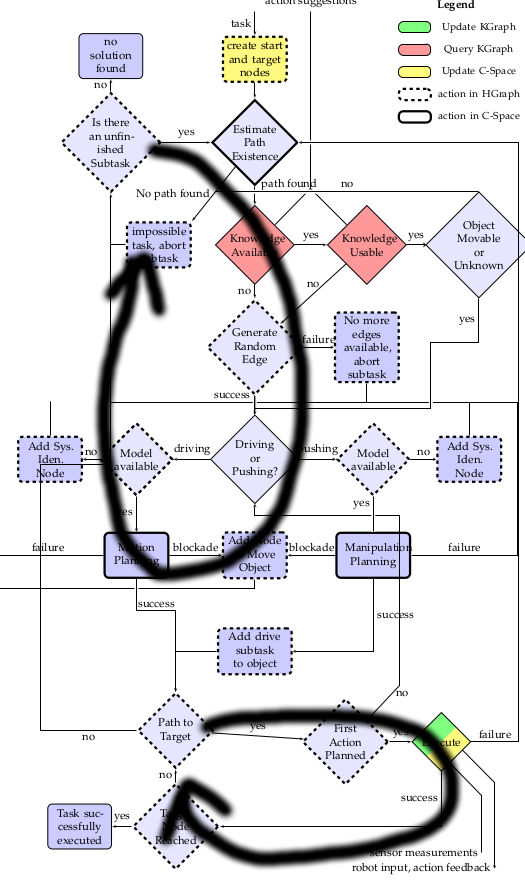
\includegraphics[width=7cm]{figures/two_loops_identified}
    \caption{The search (above) and execution (below) loop.}%
    \label{fig:two_loops_identified}
\end{figure}

Whilst the \ac{halgorithm} resides in the search loop, hypotheses are formed. Forming a hypothesis generates nodes, edges, and progressing their status as described in \cref{tikz:status_identification_edge,tikz:status_action_edge}. In the execution loop \textit{an edge is being executed}, a phrase to describe that the controller residing in an edge is sending control input toward the robot. The \ac{halgorithm} operates synchronously, thus at any point in time, the \ac{halgorithm} resides in a single block within \cref{tikz:flowchart_hgraph}. The result is that the robots cannot operate whilst the \ac{halgorithm} resides in the search loop, and during execution, no hypothesis can be formed or updated. Assumption~\ref{assumption:closed_world} guarantees that the robot environment does not change causing existing hypotheses to be outdated.\bs

\subsection{Examples}%
\label{subsec:hgraph_example}

Before displaying example \ac{hgraph}'s a legend is now presented.\bs

\begin{figure}[H]
    \centering
    \begin{subfigure}{0.2\textwidth}
    \centering
    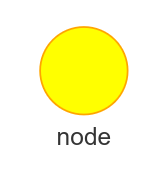
\includegraphics[width=0.7\textwidth]{figures/connecting_nodes/legend/node}
    \caption{Regular node created by the \ac{halgorithm}.\newline}%
    \end{subfigure}
    \begin{subfigure}{0.2\textwidth}
    \centering
    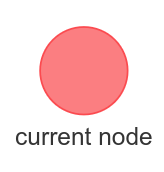
\includegraphics[width=0.7\textwidth]{figures/connecting_nodes/legend/current_node}
    \caption{Current node indicates that it's outgoing edge is now or is next to be executed.}%
    \end{subfigure}
    \begin{subfigure}{0.2\textwidth}
    \centering
    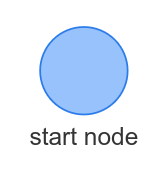
\includegraphics[width=0.7\textwidth]{figures/connecting_nodes/legend/starting_node}
    \caption{Starting node, one is generated at for every subtask.}%
    \end{subfigure}
    \begin{subfigure}{0.2\textwidth}
    \centering
    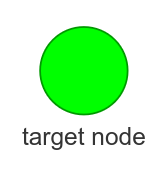
\includegraphics[width=0.7\textwidth]{figures/connecting_nodes/legend/target_node}
    \caption{Target node, one is generated for every subtask.\newline}%
    \end{subfigure}

    \begin{subfigure}{0.33\textwidth}
    \centering
    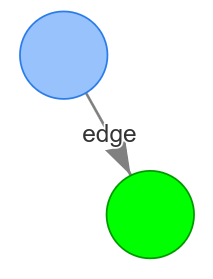
\includegraphics[width=0.7\textwidth]{figures/connecting_nodes/legend/edge}
    \caption{Edge with status IN, PE, SM, PP or EX.}%
    \end{subfigure}
    \begin{subfigure}{0.33\textwidth}
    \centering
    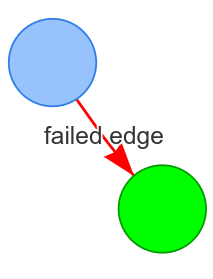
\includegraphics[width=0.7\textwidth]{figures/connecting_nodes/legend/failed_edge}
    \caption{Edge with status FAILED (FAIL)}%
    \end{subfigure}
    \begin{subfigure}{0.33\textwidth}
    \centering
    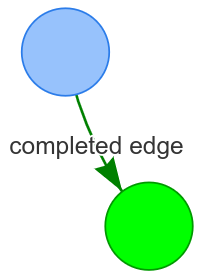
\includegraphics[width=0.7\textwidth]{figures/connecting_nodes/legend/completed_edge}
    \caption{Edge with status COMPLETED (CO)}%
    \end{subfigure}
    \caption{Legend for \ac{hgraph}'s nodes an edges}%
    \label{fig:hgraph_legend}
\end{figure}

\paragraph{Driving and Pushing} Four examples are presented, starting with a driving task in \cref{fig:robot_drive_hgraph}, then a pushing task in \cref{fig:robot_push_hgraph}.\bs

\begin{figure}[H]
    \centering
    \begin{subfigure}{.3\textwidth}
    \centering
    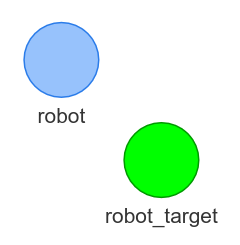
\includegraphics[width=0.7\textwidth]{figures/connecting_nodes/robot_to_target/robot_to_target}
    \end{subfigure}
    \begin{subfigure}{.3\textwidth}
    \centering
    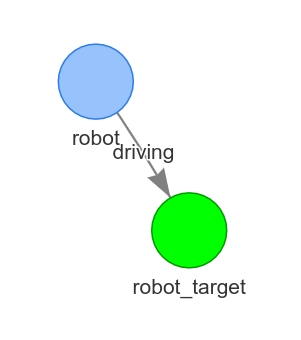
\includegraphics[width=0.9\textwidth]{figures/connecting_nodes/robot_to_target/robot_drive_target}
    \end{subfigure}
    \begin{subfigure}{.3\textwidth}
    \centering
    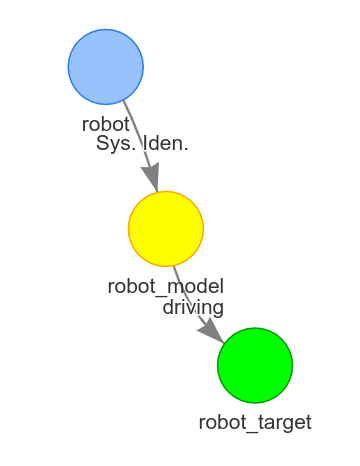
\includegraphics[width=\textwidth]{figures/connecting_nodes/robot_to_target/robot_iden_drive_target}
    \end{subfigure}
    \caption{\ac{hgraph} generated by the \ac{halgorithm} to drive the robot to a target configuration}%
    \label{fig:robot_drive_hgraph}
\end{figure}

The robot does not have a system model of itself, thus first system identification must be performed before it can drive to the specified target configuration. The \ac{kgraph} that will be discussed in \cref{subsec:kgraph_definition} can suggest an action that includes a system model. In that case, system identification is not needed. The following figure displays succesfully executing the hypothesis found in \cref{fig:robot_drive_hgraph}.\bs

\begin{figure}[H]
    \centering
    \begin{subfigure}{.3\textwidth}
    \centering
    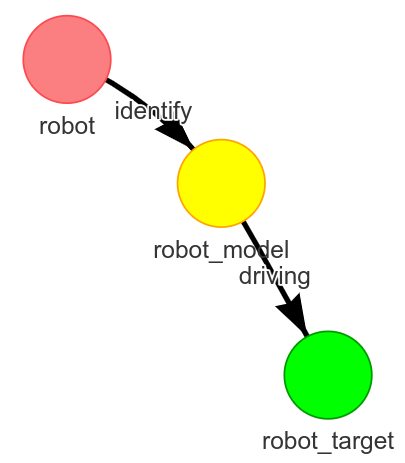
\includegraphics[width=0.8\textwidth]{figures/connecting_nodes/robot_to_target/execute_robot_to_target_1}
    \end{subfigure}
    \begin{subfigure}{.3\textwidth}
    \centering
    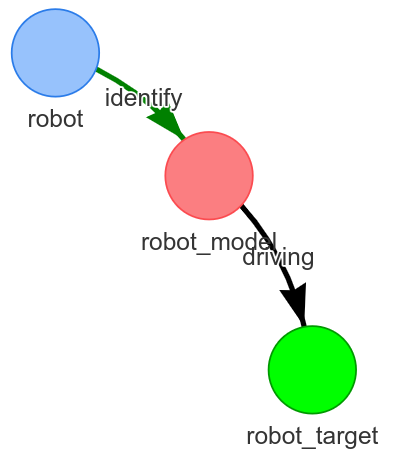
\includegraphics[width=0.8\textwidth]{figures/connecting_nodes/robot_to_target/execute_robot_to_target_2}
    \end{subfigure}
    \begin{subfigure}{.3\textwidth}
    \centering
    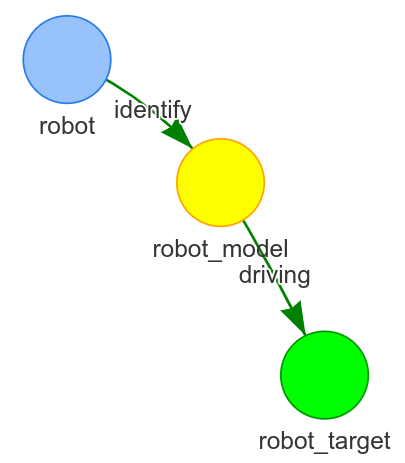
\includegraphics[width=0.8\textwidth]{figures/connecting_nodes/robot_to_target/execute_robot_to_target_3}
    \end{subfigure}
    \caption{Executing the hypothesis found in \cref{fig:robot_drive_hgraph}.}
    \label{fig:execute_robot_to_target}
\end{figure}

Upcoming figure will display the hypothesis generated to push an object to a target position. Both generating a hypothesis and executing the hypothesis are intertwined, this is because certain information should first be collected from the environment before the full hypothesis can be generated. An example is the \textit{best\_push\_position} that can be found in \cref{subfig:robot_push_7,subfig:robot_push_8,subfig:robot_push_9}. The \textit{best\_push\_position} can be found after manipulation planning for the pushing edge is completed. For motion planning a system model is required, thus the corresponding system identification edge should be completed before manipulation planning can start, and than the \textit{best\_push\_position} can be determined.\bs

\begin{figure}[H]
    \centering
    \begin{subfigure}{.3\textwidth}
    \centering
    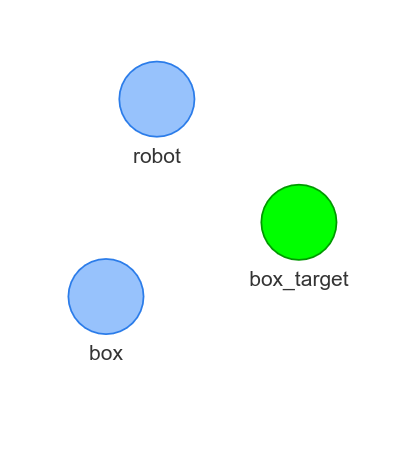
\includegraphics[width=0.8\textwidth]{figures/connecting_nodes/robot_push/robot_push_1}
    \caption{}
    \end{subfigure}
    \begin{subfigure}{.3\textwidth}
    \centering
    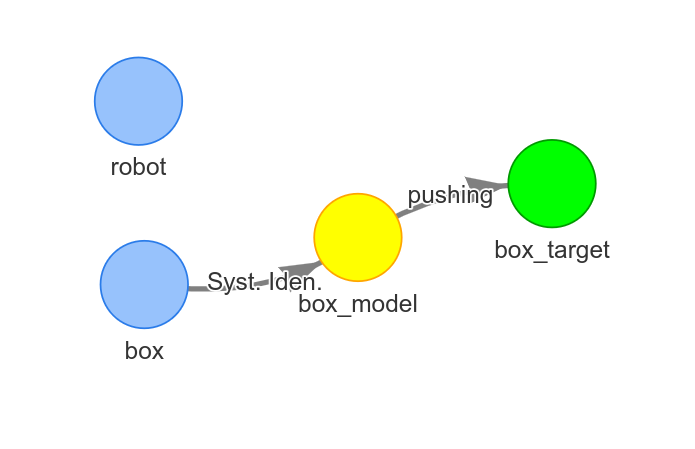
\includegraphics[width=1.1\textwidth]{figures/connecting_nodes/robot_push/robot_push_2}
    \caption{}\label{subfig:robot_push_2}
    \end{subfigure}
    \begin{subfigure}{.3\textwidth}
    \centering
    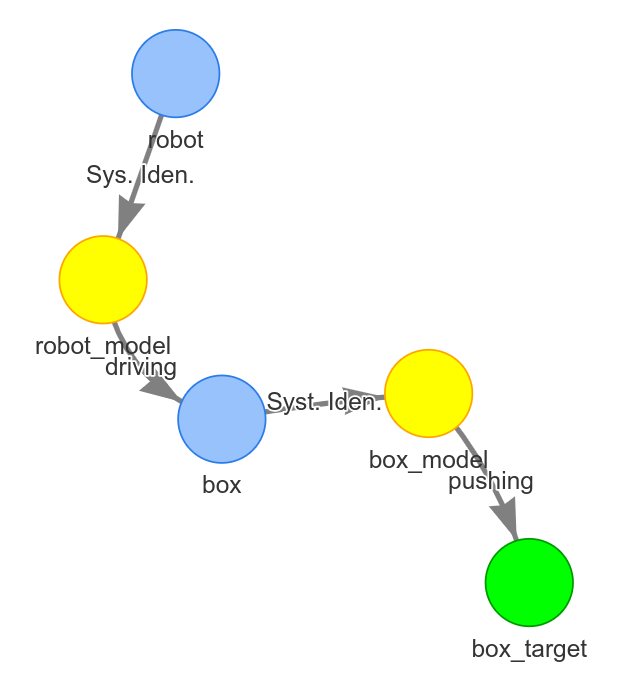
\includegraphics[width=1\textwidth]{figures/connecting_nodes/robot_push/robot_push_3}
    \caption{}\label{subfig:robot_push_3}
    \end{subfigure}

    \begin{subfigure}{.3\textwidth}
    \centering
    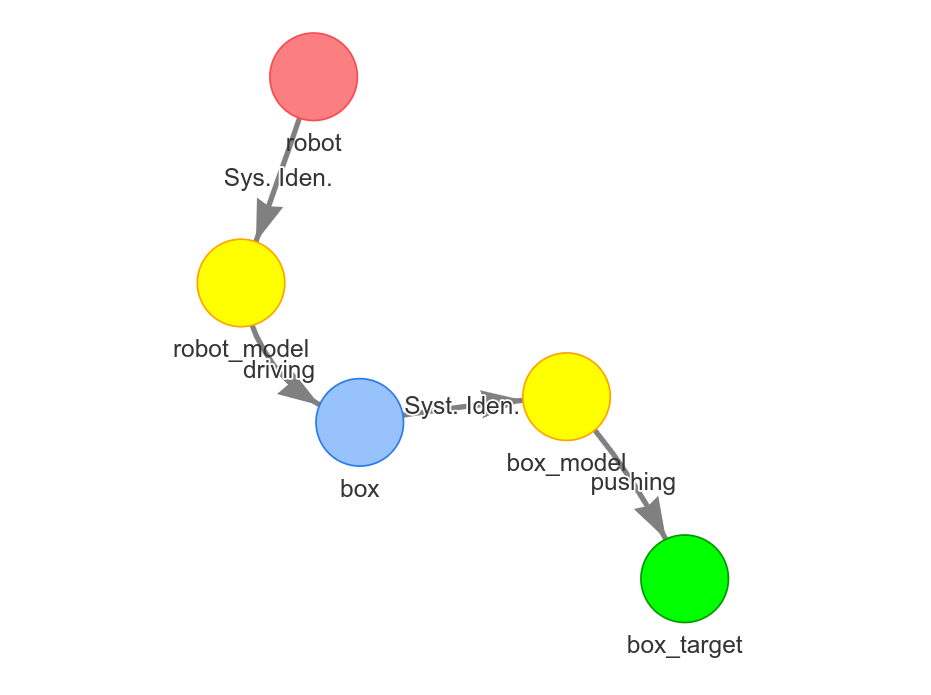
\includegraphics[width=1\textwidth]{figures/connecting_nodes/robot_push/robot_push_4}
    \caption{}\label{subfig:robot_push_4}
    \end{subfigure}
    \begin{subfigure}{.3\textwidth}
    \centering
    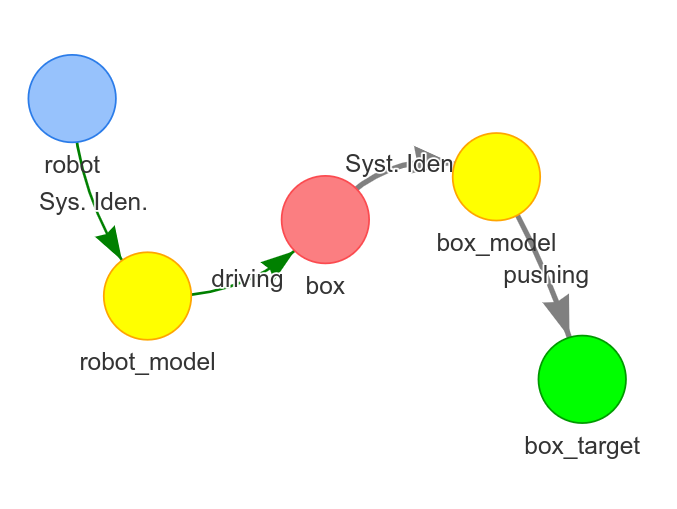
\includegraphics[width=1.05\textwidth]{figures/connecting_nodes/robot_push/robot_push_5}
    \caption{}\label{subfig:robot_push_5}
    \end{subfigure}
    \begin{subfigure}{.3\textwidth}
    \centering
    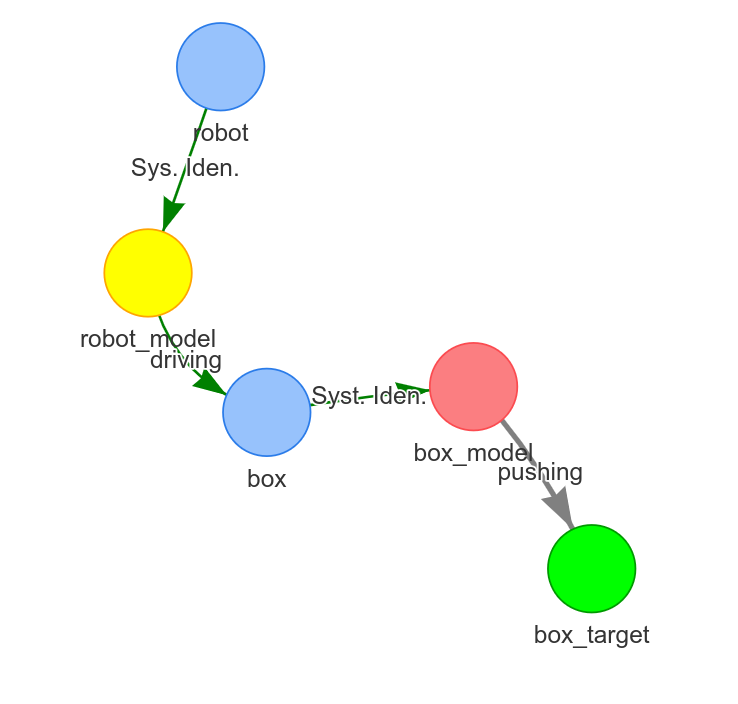
\includegraphics[width=1.05\textwidth]{figures/connecting_nodes/robot_push/robot_push_6}
    \caption{}\label{subfig:robot_push_6}
    \end{subfigure}

    \begin{subfigure}{.3\textwidth}
    \centering
    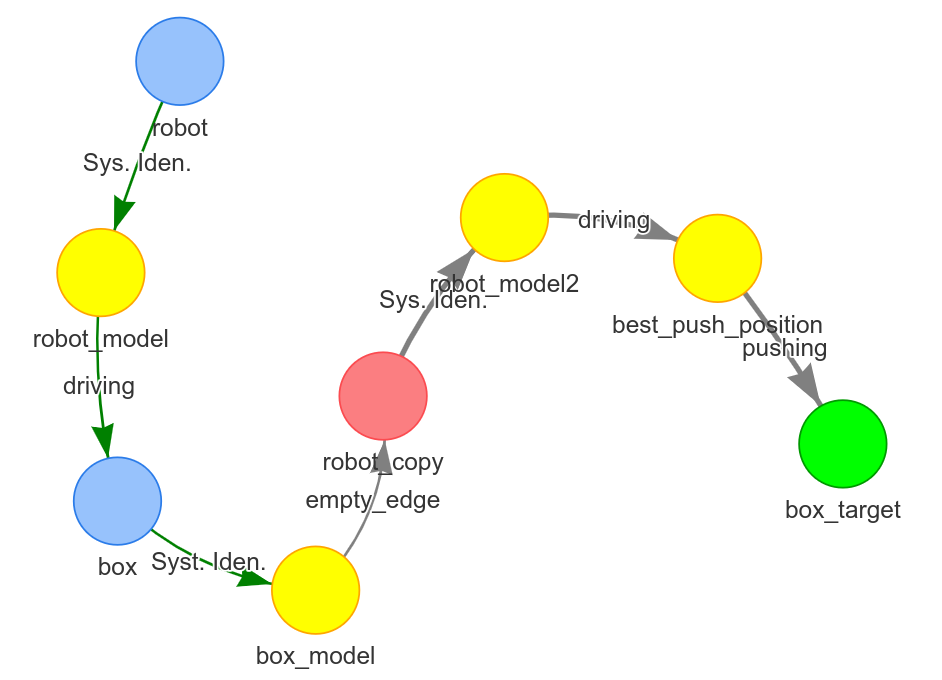
\includegraphics[width=1\textwidth]{figures/connecting_nodes/robot_push/robot_push_7}
    \caption{}\label{subfig:robot_push_7}
    \end{subfigure}
    \begin{subfigure}{.3\textwidth}
    \centering
    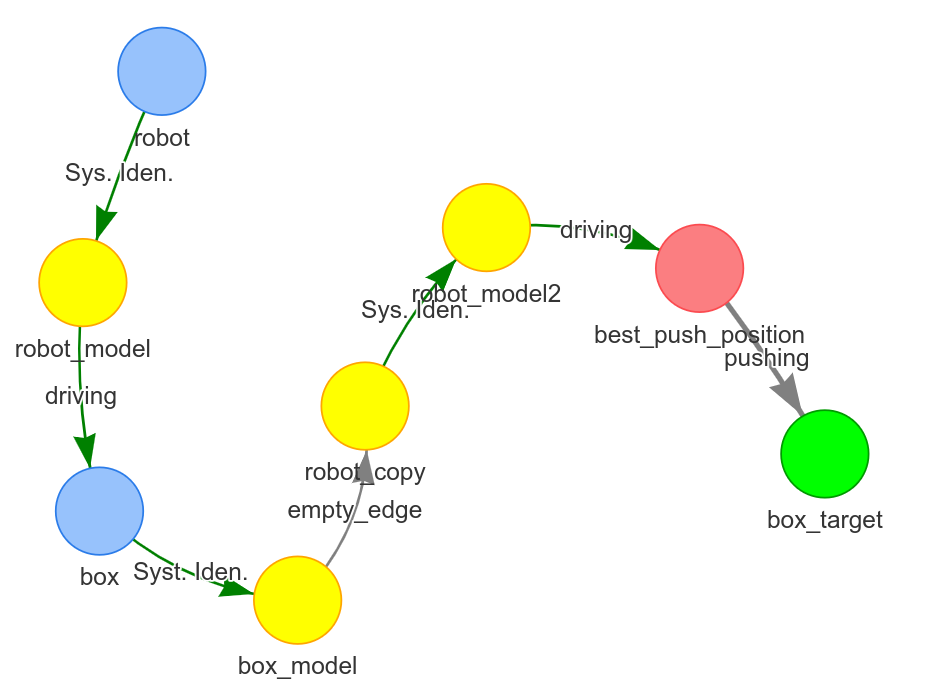
\includegraphics[width=1.05\textwidth]{figures/connecting_nodes/robot_push/robot_push_8}
    \caption{}\label{subfig:robot_push_8}
    \end{subfigure}
    \begin{subfigure}{.3\textwidth}
    \centering
    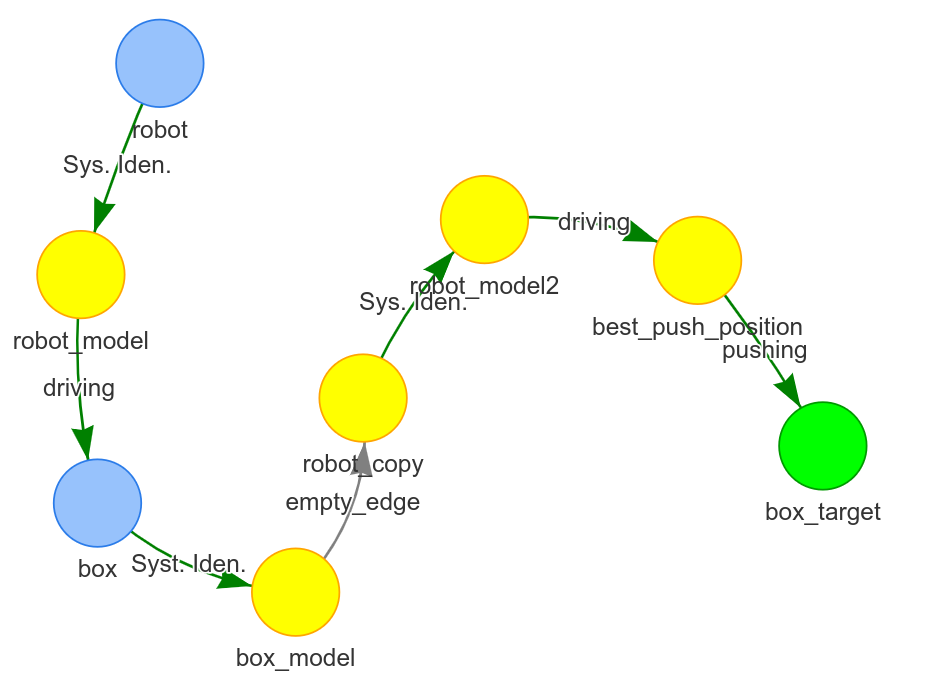
\includegraphics[width=1.05\textwidth]{figures/connecting_nodes/robot_push/robot_push_9}
    \caption{}\label{subfig:robot_push_9}
    \end{subfigure}
    \caption{\ac{hgraph} for pushing the green box to the target configuration}%
    \label{fig:robot_push_hgraph}
\end{figure}
Especially in \cref{subfig:robot_push_2,subfig:robot_push_3} the backward search is clearly visible, the \ac{halgorithm} searches from target node to the robot node. \Cref{fig:robot_push_hgraph} is extensive because every nessecary steps is included whilst some could be skipped. First, identifying a system model for robot driving twice, if the system model created in edge Sys. Iden. pointing toward node robot\_model is reused, then the edge Sys. Iden. pointing toward robot\_model\_1 would be unnecessary. Second, if system models would already be availeble for driving and pushing, no single system identification edge would be required. A \textit{empty\_edge} can be seen in \cref{subfig:robot_push_7,subfig:robot_push_8,subfig:robot_push_9}, the empty\_edge serves to connect a node to another node (box\_model to robot\_copy in \cref{fig:robot_push_hgraph}). The empty\_edge can be traversed without execution, holds no controller, system model or status.\bs

\paragraph{Encountering a Blocked Path}%
During propagation of an action edge's status, motion or manipulation planning occurs. If an object is blocking the path, planning will detect it and the \ac{halgorithm} tries to free the path. In the next example the \ac{halgorithm} detects a blocking object and frees the path by pushing the blocking object to a new configuration, and can be visulised in \cref{fig:blocking_obj_hgraph}.\bs

\begin{figure}[H]
    \centering
    \begin{subfigure}{.3\textwidth}
    \centering
    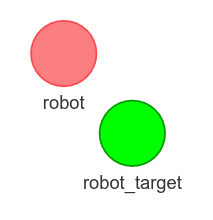
\includegraphics[width=0.5\textwidth]{figures/connecting_nodes/blocking_obj/blocking_obj_1}
    \caption{}
    \end{subfigure}
    \begin{subfigure}{.3\textwidth}
    \centering
    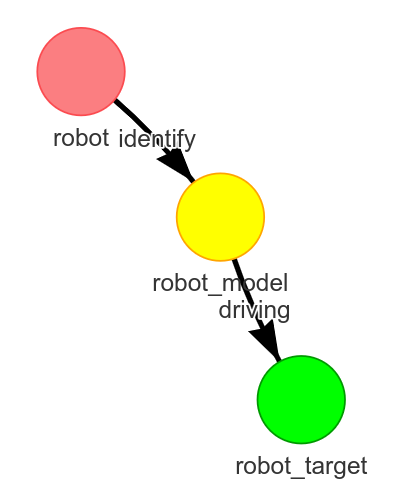
\includegraphics[width=\textwidth]{figures/connecting_nodes/blocking_obj/blocking_obj_2}
    \caption{}\label{subfig:blocking_obj_2}
    \end{subfigure}
    \begin{subfigure}{.3\textwidth}
    \centering
    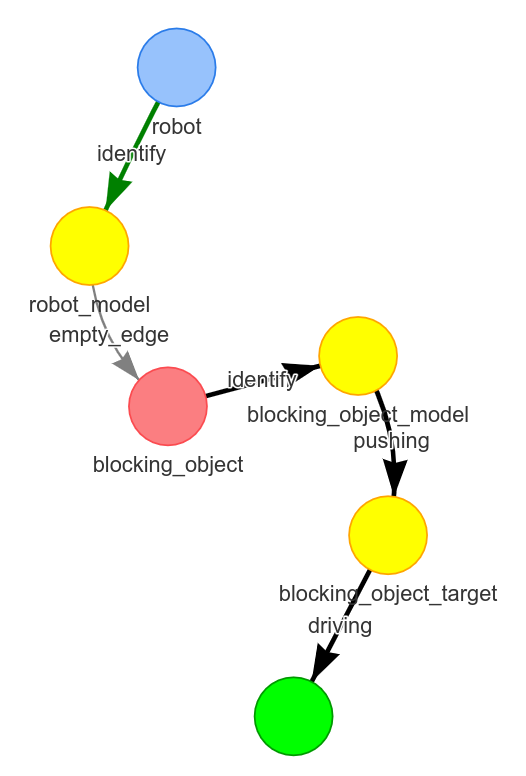
\includegraphics[width=\textwidth]{figures/connecting_nodes/blocking_obj/blocking_obj_3}
    \caption{}\label{subfig:blocking_obj_3}
    \end{subfigure}

    \begin{subfigure}{.3\textwidth}
    \centering
    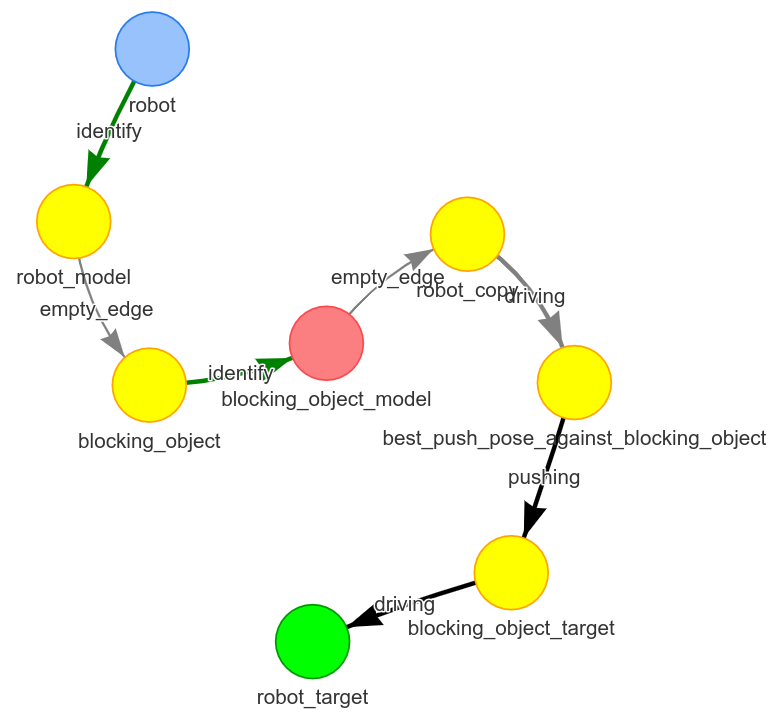
\includegraphics[width=1.3\textwidth]{figures/connecting_nodes/blocking_obj/blocking_obj_4}
    \caption{}\label{subfig:blocking_obj_4}
    \end{subfigure}
    \begin{subfigure}{.3\textwidth}
    \centering
    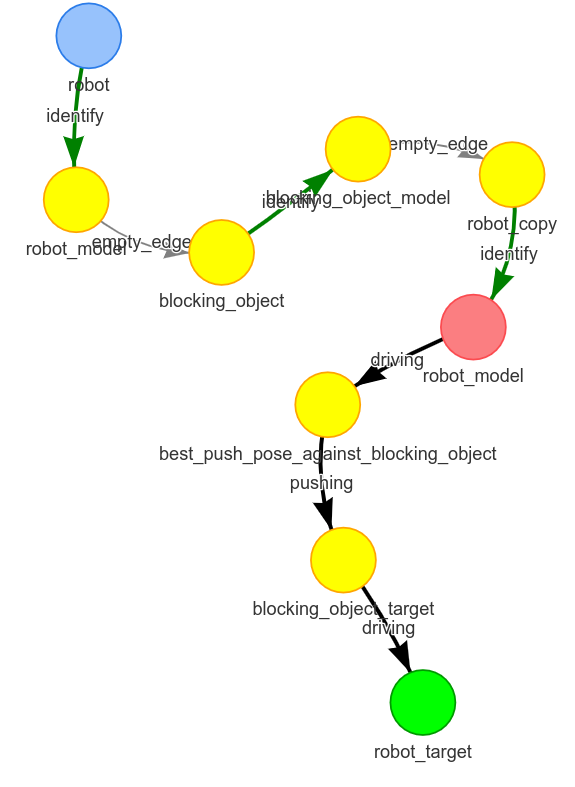
\includegraphics[width=\textwidth]{figures/connecting_nodes/blocking_obj/blocking_obj_5}
    \caption{}\label{subfig:blocking_obj_5}
    \end{subfigure}
    \begin{subfigure}{.3\textwidth}
    \centering
    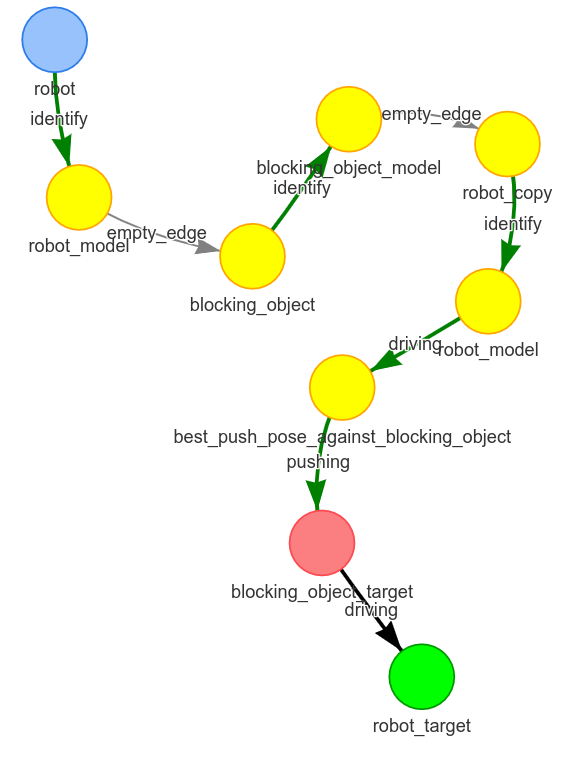
\includegraphics[width=\textwidth]{figures/connecting_nodes/blocking_obj/blocking_obj_6}
    \caption{}\label{subfig:blocking_obj_6}
    \end{subfigure}
    \caption{\ac{hgraph} for driving to target configuration and encountering a blocked path}%
    \label{fig:blocking_obj_hgraph}
\end{figure}

\paragraph{Encountering Failure}%
In the last example, the first hypothesis fails to complete and the \ac{halgorithm} tries to generate a new hypothesis that also fails to complete. Several faults and failures are modelled, the \ac{halgorithm} response to faults and failure is the same. If during the propagation of an edge's status any kind of failure arises, the failed edge and corresponding edges are marked as failed. Equally during execution, if a fault is detected, the execution halts and the edge and corresponding edges are marked as \quotes{failed}, the procedure can be seen in \cref{fig:failure_in_hgraph}.\bs

\begin{figure}[H]
    \centering
    \begin{subfigure}{.3\textwidth}
    \centering
    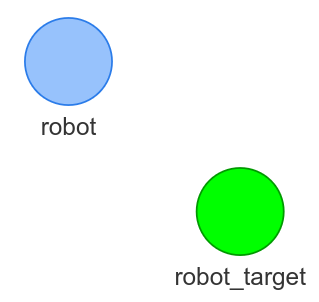
\includegraphics[width=0.8\textwidth]{figures/connecting_nodes/failure/fail_1}
    \end{subfigure}
    \begin{subfigure}{.3\textwidth}
    \centering
    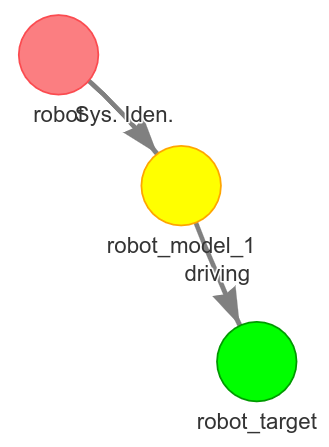
\includegraphics[width=1.1\textwidth]{figures/connecting_nodes/failure/fail_2}
    \end{subfigure}
    \begin{subfigure}{.3\textwidth}
    \centering
    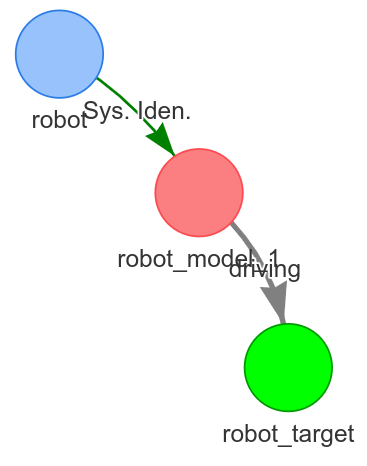
\includegraphics[width=1\textwidth]{figures/connecting_nodes/failure/fail_3}
    \end{subfigure}

    \begin{subfigure}{.3\textwidth}
    \centering
    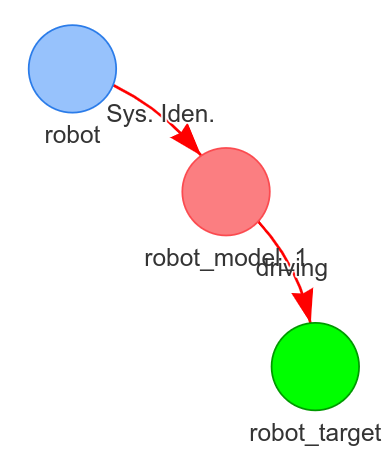
\includegraphics[width=1\textwidth]{figures/connecting_nodes/failure/fail_4}
    \end{subfigure}
    \begin{subfigure}{.3\textwidth}
    \centering
    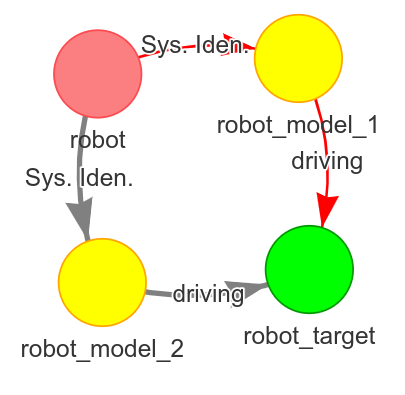
\includegraphics[width=1\textwidth]{figures/connecting_nodes/failure/fail_5}
    \end{subfigure}
    \begin{subfigure}{.3\textwidth}
    \centering
    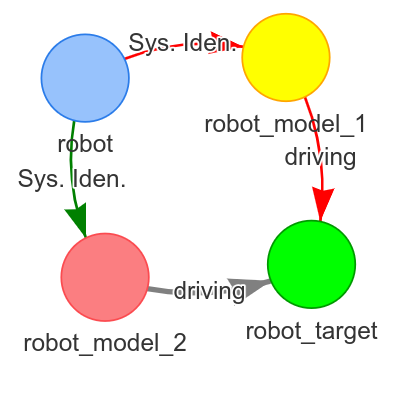
\includegraphics[width=1\textwidth]{figures/connecting_nodes/failure/fail_6}
    \end{subfigure}

    \begin{subfigure}{.3\textwidth}
    \centering
    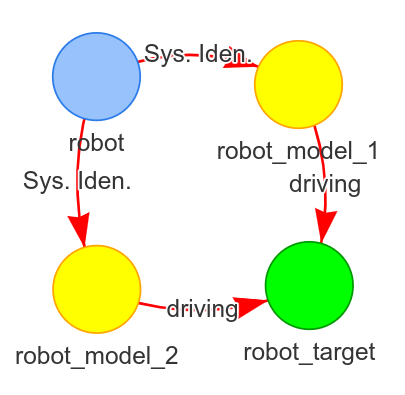
\includegraphics[width=1\textwidth]{figures/connecting_nodes/failure/fail_7}
    \end{subfigure}
    \hfill
    \caption{Executing two hypothesis, both failing to complete because a fault of failure emerged.}%
    \label{fig:failure_in_hgraph}
\end{figure}

In \cref{fig:failure_in_hgraph} only two parameterisations of drive controller and system model were available. Thus after two failed hypothesis the \ac{halgorithm} concludes it cannot complete this task.\bs


What by now hopefully became clear to the reader is that the \ac{halgorithm} autonomously searches for hypotheses in the \ac{hgraph} to solve a task, one subtask at a time. The \ac{halgorithm} switches between the search and execution loop. Switching from the search loop toward the execution loop when a hypothesis is found, and switching back when a hypothesis is completed or an fault or failure occurred.\bs

The limited number of possible edge parameterisations (every combination of a system identification method with a compatible control method) guarantees that the robot tries to complete a subtask, but concludes that it is unable to complete a subtask if all possible edges have failed.\bs

Recall the 3 topics (learning object dynamics, the \ac{NAMO} problem and nonprehensile push manipulation) that this thesis proposes to combine. The \ac{halgorithm} can solve \ac{NAMO} problems because the robot can drive toward target positions even if reaching such a position requires objects to be moved first. The \ac{halgorithm} can push objects to target positions by first identifying a system model and then pushing the object toward its target position. The proposed algorithm learns to classify objects by updating objects class from unknown to movable or obstacle. The system model that system identification yields is however of short use, it is only given to the corresponding action edge. In the next section, the edges that are executed will be reviewed and stored in a knowledge base. The knowledge base will suggest a parameterisation for an edge when faced with similar nodes to connect. 
